\chapter{Subspace Identification Methods}\label{theory}
Subspace identification methods provide an approach to identifing LTI systems in their state space form using input-output data. SIMs provide an attractive alternative to prediction error methods because of their ability to identify MIMO systems and because of their non-iterative solution nature, making them suitable for working with large data sets. In general, the subspace identification problem is: given a set of system input and output data, estimate the system matrices ($A$, $B$, $C$, $D$) up to within a similarity transform. 

Extensive work in both the theory and application of SIMs in the last 20 years has resulted in the development of a number of popular algorithms, including the canonical variate analysis (CVA) method proposed by Larimore \cite{larimore1990canonical}, the multi-variable output-error state space (MOESP) method proposed by Verhaegen \cite{verhaegen1992subspace}, and the numerical algorithms for subspace state space system identification (N4SID) proposed by Van Overschee and De Moor \cite{van1994n4sid}. A unifying theorem subsequently proposed by Van Overschee and De Moor \cite{van1995unifying} links these algorithms and provides a generalized approach to the subspace identification problem by assigning different weighting matrices for each method.

As described in Van Overschee and De Moor's unifying theorem, all SIMs follow the same general two step procedure. First, estimate the subspace spanned by the columns of the extended observability matrix ($\Gamma_k$) from input-output data $u_k$ and $y_k$. Because the dimension of $\Gamma_k$ determines the order $n$ of the estimated system, a reduction of the system order is performed before proceeding. Second, the system matrices are determined, either directly from the extended observability matrix or from the realized state sequence $X_k$.
\begin{figure}[htb!]
	\centering
	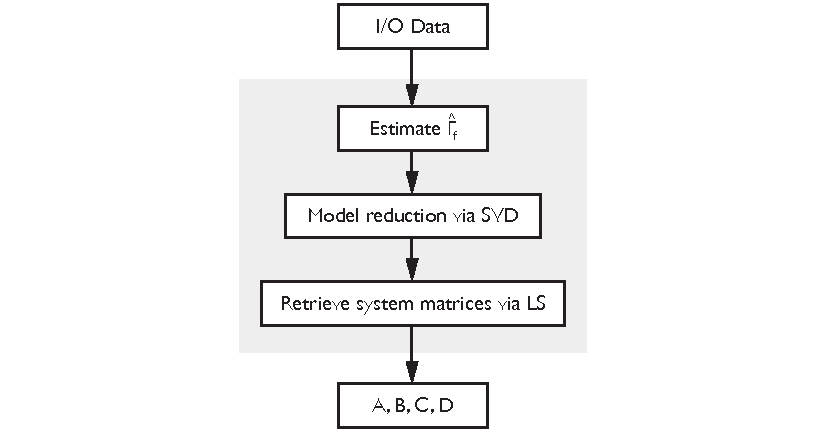
\includegraphics{../fig/sim_flow_diagram.pdf}
	\caption{Subspace identification approach}
\end{figure}

\section{Subspace System Identification}
First, we consider the identification of a combined deterministic-stochastic LTI system operating in open loop.
\begin{figure}[htb!]
	\centering
	
\includegraphics{../fig/open_loop_block_diagram.pdf}
	\caption{A block diagram of an LTI system operating in open loop.}
\end{figure}
We present an overview of the PO-MOESP subspace identification procedure, where ``PO'' stands for past output, indicating that both past input and output data is used when eliminating the influence of noise on the identified system, further described in Sec. \ref{sec:estimation_of_the_extended_observability_matrix}. Before detailing the identification procedure, we introduce the following assumptions:\\
\textbf{Assumption 1}: The matrix $A - KC$ is stable (i.e. its eigenvalues lie strictly within the unit circle).\\
\textbf{Assumption 2}: The pair $(A,C)$ is observable and $(A, [B \quad K])$ is controllable.\\
\textbf{Assumption 3}: The innovation sequence $e(k)$ can be modeled as zero-mean white-noise.\\
\textbf{Assumption 4}: The input sequence $u(k)$ and innovation sequence $e(k)$ are uncorrelated for all $k$.\\
\textbf{Assumption 5}: The input sequence $u(k)$ is persistently exciting.

\subsection{Extended State Space Model}\label{sec:extended_state_space_model}
Recalling the combined deterministic-stochastic LTI system is given in its innovation form as
\begin{subequations}
\begin{equation}x(k+1) = Ax(k) + Bu(k) + Ke(k)\end{equation}
\begin{equation}y(k) = Cx(k) + Du(k) + e(k)\end{equation}
\end{subequations}
Based on the state space representation, an extended state space model can be formulated as
\begin{subequations}
\begin{equation}Y_p = \Gamma_p X_{k-p} + H_p U_p + G_p E_p\end{equation}
\begin{equation}Y_f = \Gamma_f X_k + H_f U_f + G_f E_f\label{eq:3_extended-State_space_future_horizon}\end{equation}
\end{subequations}
where $p$ and $f$ denote past and future horizons, respectively. Considering the future horizon given in Eq. \ref{eq:3_extended-State_space_future_horizon}, the extended observability matrix is
\begin{equation*}
\Gamma_f = \begin{bmatrix}C\\ CA\\ \vdots\\ CA^{f-1}\end{bmatrix}
\end{equation*}
and $H_f$ and $G_f$ are Toeplitz matrices of the Markov parameters of the deterministic and stochastic subsystems, respectively:
\begin{equation*}
H_f = \begin{bmatrix}
D & 0 & 0 & \cdots & 0\\
CB & D & 0 & \cdots & 0\\
CAB & CB & D & \cdots & 0\\
\vdots & \vdots  & \vdots & \ddots & \vdots\\
CA^{f-2}B & CA^{f-3}B & CA^{f-4}B & \cdots & D
\end{bmatrix}
\end{equation*}
\begin{equation*}
G_f = \begin{bmatrix}
I & 0 & 0 & \cdots & 0\\
CK & I & 0 & \cdots & 0\\
CAK & CK & I & \cdots & 0\\
\vdots & \vdots  & \vdots & \ddots & \vdots\\
CA^{f-2}K & CA^{f-3}K & CA^{f-4}K & \cdots & I
\end{bmatrix}
\end{equation*}
We arrange the past and future input sequences into the following block Hankel form with $k$ block rows and $N$ columns:
\begin{equation*}
U_p = \begin{bmatrix}
u(0) & u(1) & \cdots & u(N-1)\\
u(1) & u(2) & \cdots & u(N)\\
\vdots & \vdots & \ddots & \vdots\\
u(k-1) & u(k) & \cdots & u(k+N-2)
\end{bmatrix}
\end{equation*}
\begin{equation*}
U_f = \begin{bmatrix}
u(k) & u(k+1) & \cdots & u(k+N-1)\\
u(k+1) & u(k+2) & \cdots & u(k+N)\\
\vdots & \vdots & \ddots & \vdots\\
u(2k-1) & u(2k) & \cdots & u(2k+N-2)
\end{bmatrix}
\end{equation*}
We construct similar matrices $Y_p$, $Y_f$, $E_p$, and $E_f$ for the output and noise sequences. The state sequences are
\begin{equation*}
X_k = \begin{bmatrix}
x(k) & x(k+1) & \cdots & x(k+N-1)
\end{bmatrix}
\end{equation*}
\begin{equation*}
X_{k-p} = \begin{bmatrix}
x(k-p) & x(k-p+1) & \cdots & x(k-p+N-1)
\end{bmatrix}
\end{equation*}
We will leverage this structure of the extended state space model to identify the unknown system matrices from known input-output data. In particular, we will estimate the column space of the extended observability matrix. Knowledge of this subspace is sufficient to then recover the unknown system matrices. 


\subsection{Estimation of the Extended Observability Matrix}\label{sec:estimation_of_the_extended_observability_matrix}
Determination of the system matrices relies on an estimate of the column space of $\Gamma_f$. Recalling the extended state space model and again considering only the future horizon, we have
\begin{equation}\label{eq:3_extended_state_space_future}
Y_f = \Gamma_f X_k + H_f U_f + G_f E_f
\end{equation}
In order to estimate the column space of the extended observability matrix $\Gamma_f$ in Eq. (\ref{eq:3_extended_state_space_future}), we must eliminate the influence of the input sequence $U_f$ and noise term $E_f$. The general procedure, as outlined in \cite{qin2006overview, verhaegen2007filtering} is as follows: First, we eliminate the influence of the input $U_f$ by multiplying Eq. (\ref{eq:3_extended_state_space_future}) on the right by $\Pi_{U_f}^\perp$ where $\Pi_{U_f}^\perp$ is an orthogonal projection onto the column space of $U_f$ given by
\begin{equation*}
\Pi_{U_f}^\perp = I - U_f^T(U_f U_f^T)^{-1}U_f
\end{equation*}
By definition, $U_f\Pi_{U_f}^\perp = 0$ so Eq. (\ref{eq:3_extended_state_space_future}) becomes
\begin{equation}
Y_f\Pi_{U_f}^\perp = \Gamma_f X_k\Pi_{U_f}^\perp + G_f E_f\Pi_{U_f}^\perp
\end{equation}
By Assumption 4, the noise term $E_f$ is uncorrelated with the input sequence $U_f$. That is,
\begin{equation*}
E_f \Pi_{U_f}^\perp = E_f(I-U_f^T(U_fU_f^T)^{-1}U_f) = E_f
\end{equation*}
so
\begin{equation}\label{eq:3_extended_state_space_noinput}
Y_f\Pi_{U_f}^\perp = \Gamma_f X_k\Pi_{U_f}^\perp + G_f E_f
\end{equation}
Next we eliminate the influence of the noise $E_f$. In order to remove the influence of the noise on the extended observability matrix, we must introduce an instrumental variable matrix as described in \cite{verhaegen2007filtering}. We seek a matrix $Z_i \in \mathbb{R}^{2k\times N}$ which exhibits the following properties:
\begin{subequations}\begin{equation}\label{eq:3_instrumental_a}
\lim_{N\rightarrow\infty} \frac{1}{N} E_f Z_i^T = 0
\end{equation}
\begin{equation}\label{eq:3_instrumental_b}
\mbox{rank}\left(\lim_{N\rightarrow\infty} \frac{1}{N} X_k \Pi_{U_f}^\perp Z_i^T\right) = n
\end{equation}
\end{subequations}
Satisfying condition (\ref{eq:3_instrumental_a}) ensures that we can eliminate the noise term $E_f$ by multiplying Eq. (\ref{eq:3_extended_state_space_noinput}) on the right by $Z_i^T$ and taking the limit for $N\rightarrow\infty$:
\begin{equation}\label{eq:3_extended_state_space_noinput_nonoise}
\lim_{N\rightarrow\infty} \frac{1}{N}Y_f\Pi_{U_f}^\perp Z_i^T = \lim_{N\rightarrow\infty} \frac{1}{N}\Gamma_f X_k\Pi_{U_f}^\perp Z_i^T
\end{equation}
 Satisfying condition (\ref{eq:3_instrumental_b}) ensures multiplication by $Z_i$ does not change the rank of the remaining term on the right hand side of Eq. (\ref{eq:3_extended_state_space_noinput_nonoise}) so we have
\begin{equation}\label{eq:3_range}
\mbox{range}\left(\lim_{N\rightarrow\infty} \frac{1}{N} Y_f\Pi_{U_f}^\perp Z_i^T\right) = \mbox{range}\left(\Gamma_f\right)
\end{equation}
From Eq. (\ref{eq:3_range}) we see that an SVD of the matrix $Y_f\Pi_{U_f}^\perp Z_i^T$  will provide an estimate of the column space of $\Gamma_f$. All that remains is to identify a suitable instrumental variable matrix $Z_i$. As described in \cite{soderstrom1983instrumental, verhaegen2007filtering}, instrumental variable matrices are typically constructed from input-output data. Recalling that we partitioned the input and output data into past and future sets in Section \ref{sec:extended_state_space_model}, we will use the future input-output data to identify the system and the past input-output data as the instrumental variable matrix, called $Z_p$:
\begin{equation*}
Z_p = \begin{bmatrix}U_p\\ Y_p\end{bmatrix}
\end{equation*}
Recalling that the noise $E_f$ is uncorrelated with the input $U_f$ for open-loop systems, and enforcing the assumption that $E_f$ is white-noise, we have from \cite{verhaegen2007filtering} that 
\begin{equation*}
\lim_{N\rightarrow\infty} \frac{1}{N} E_f Z_p^T = 0
\end{equation*}
which satisfies condition (\ref{eq:3_instrumental_a}). Jannson showed in \cite{jansson1997subspace} that if the input sequence is persistently exciting (Assumption 5), the rank condition (\ref{eq:3_instrumental_b}) on the instrumental variable matrix is satisfied. Taking $Z_p$ as the instrumental variable matrix and taking the SVD, from Eq. (\ref{eq:3_range}) we have
\begin{equation}
\hat{\Gamma}_f = U {S}^{1/2}
\end{equation}


\subsection{Rank Reduction}\label{sec:3_rank_reduction}
In the presence of noise, the matrix $Y_f\Pi_{U_f}^\perp Z_p^T$ is full rank while the true system order is smaller. We choose the order of the identified system by partitioning the SVD matrices as follows:
\begin{equation*}
Y_f\Pi_{U_f}^\perp Z_p^T = 
\begin{bmatrix}U_1 & U_2\end{bmatrix}
\begin{bmatrix}S_1 & 0\\ 0 & S_2\end{bmatrix}
\begin{bmatrix}V_1^T & V_2^T\end{bmatrix}
\end{equation*}
where the number of singular values $n$ in $S_1$ is equal to the system order and the remaining submatrices are scaled appropriately. Selecting only the most significant singular values for inclusion in the estimate ensures the true system dynamics are captured while reducing the inclusion of noise. The reduced rank estimate of the extended observability matrix is then
\begin{equation}
\hat{\Gamma}_f = U_1 {S_1}^{1/2}
\end{equation}


\subsection{Determination of the System Matrices}\label{sec:3_system_matrices}
With an estimate of the column space of $\Gamma_f$, we are now able to recover the system matrices. In order to recover the system matrices, we follow the general procedure as outlined in \cite{katayama2005subspace}. First, we will exploit the structure of the extended observability matrix to recover the $A$ and $C$ matrices. The matrix $C$ can be read directly from the first block row of $\hat{\Gamma}_f$. In order to recover $A$, we define the following two modified extended observability matrices:
\begin{equation}\label{eq:3_shifted_gamma}
\hat{\overline{\Gamma}}_f = \begin{bmatrix}C\\ \vdots \\ CA^{f-2}\end{bmatrix}, \hspace{3em}
\hat{\underline{\Gamma}}_f = \begin{bmatrix}CA\\ \vdots \\ CA^{f-1}\end{bmatrix}
\end{equation}
where $\hat{\overline{\Gamma}}_f$ is equal to $\hat{\Gamma}_f$ without the last block row and $\hat{\underline{\Gamma}}_f$ is equal to $\hat{\Gamma}_f$ without the first block row. The structure of the matrices in Eq. (\ref{eq:3_shifted_gamma}) implies
\begin{equation}
\hat{\overline{\Gamma}}_f A = \hat{\underline{\Gamma}}_f
\end{equation}
which is linear in $A$ and can be solved by least squares.

All that remains is to recover the $B$ and $D$ matrices. We follow the general procedure outlined in \cite{trnka2007subspace}. Recalling the extended state space model is given by
\begin{equation*}
Y_f = \Gamma_f X_k + H_f U_f + G_f E_f
\end{equation*}
and multiplying on the left by $\hat{\Gamma}_f^\perp$ and on the right by ${U_f}^\dagger$ we have
\begin{equation}\label{eq:3_extended_state_space_bd}
\hat{\Gamma}_f^\perp Y_f {U_f}^\dagger = \hat{\Gamma}_f^\perp\Gamma_f X_k {U_f}^\dagger + \hat{\Gamma}_f^\perp H_f U_f {U_f}^\dagger + \hat{\Gamma}_f^\perp G_f E_f {U_f}^\dagger
\end{equation}
where $\hat{\Gamma}_f^\perp$ satisfies $\hat{\Gamma}_f^\perp\hat{\Gamma}_f = 0$ and $\dagger$ denotes the Moore-Penrose pseudoinverse where $U_f U_f^\dagger = 1$. Equation (\ref{eq:3_extended_state_space_bd}) simplifies to
\begin{equation}\label{eq:3_extended_state_space_bd_simplified}
\hat{\Gamma}_f^\perp Y_f {U_f}^\dagger = \hat{\Gamma}_f^\perp H_f 
\end{equation}
Partitioning $\hat{\Gamma}_f^\perp Y_f {U_f}^\dagger$ into columns with the $i^{\mbox{th}}$ column denoted by $\mathcal{M}_i$ and $\hat{\Gamma}_f^\perp$ into rows with the $j^{\mbox{th}}$ row denoted by $\mathcal{L}_j$, Eq. (\ref{eq:3_extended_state_space_bd_simplified}) is
\begin{equation*}
\begin{bmatrix}\mathcal{M}_1 & \mathcal{M}_2 & \cdots & \mathcal{M}_f\end{bmatrix} = 
\begin{bmatrix}\mathcal{L}_1\\ \mathcal{L}_2\\ \vdots\\ \mathcal{L}_f\end{bmatrix}
\begin{bmatrix}
D & 0 & \cdots & 0\\
CB & D & \cdots & 0\\
\vdots & \vdots  & \ddots & \vdots\\
CA^{f-2}B & CA^{f-3}B & \cdots & D
\end{bmatrix}
\end{equation*}
We can rewrite the above equation as
\begin{equation}
\begin{bmatrix}\mathcal{M}_1\\ \mathcal{M}_2\\ \mathcal{M}_3\\ \vdots\\ \mathcal{M}_f\end{bmatrix} = 
\begin{bmatrix}
\mathcal{L}_1 & \mathcal{L}_2 & \cdots & \mathcal{L}_{f-1} & \mathcal{L}_f\\
\mathcal{L}_2 & \mathcal{L}_3 & \cdots & \mathcal{L}_{f} & 0\\
\mathcal{L}_3 & \mathcal{L}_4 & \cdots & 0 & 0\\
\vdots & \vdots & \ddots & \vdots & \vdots\\
\mathcal{L}_f & 0 & 0 & \cdots & 0
\end{bmatrix}
\begin{bmatrix}I & 0\\ 0 & \hat{\overline{\Gamma}}_f\end{bmatrix}
\begin{bmatrix}D \\ B\end{bmatrix}
\end{equation}
which is an overdetermined linear system in $B$ and $D$. We recover $B$ and $D$ through least squares.


\subsection{Numerical Efficiencies by LQ Factorization}
In the case where $N$ is large, the construction of the matrix $Y_f\Pi_{U_f}^\perp Z^T$ in Eq. (\ref{eq:3_range}) and the subsequent calculation of its SVD are computationally intensive. Verhaegen showed in \cite{verhaegen1994identification} that from the following LQ decomposition
\begin{equation}\label{eq:3_lq}
\begin{bmatrix}U_f\\ U_p\\ Y_p\\ Y_f\end{bmatrix} = 
\begin{bmatrix}
	L_{11} & 0 & 0 & 0\\
	L_{21} & L_{22} & 0 & 0\\
	L_{31} & L_{32} & L_{33} & 0\\
	L_{41} & L_{42} & L_{43} & L_{44}
\end{bmatrix}
\begin{bmatrix}Q_1\\ Q_2\\ Q_3\\ Q_4\end{bmatrix}
\end{equation}
we have
\begin{equation}\label{eq:3_range_lq}
\mbox{range}\left(\lim_{N\rightarrow\infty} \frac{1}{\sqrt{N}} \begin{bmatrix}L_{42} & L_{43}\end{bmatrix}\right) = \mbox{range}\left(\Gamma_f\right)
\end{equation}
This result illustrates the equivalency between Eq. (\ref{eq:3_range}) and Eq. (\ref{eq:3_range_lq}), therefore we can estimate the column space of $\hat{\Gamma}_f$ by computing the LQ decomposition in Eq. (\ref{eq:3_lq}), taking the SVD of the matrix $\begin{bmatrix}L_{42} & L_{43}\end{bmatrix}$, and reducing the system order as described previously.









\section{Closed-Loop Subspace Identification with Innovation Estimation}\label{sec:closed-loop_subspace_identification}
In many real-world situations, it is either not practical or not possible to collect open-loop input and output data. An unstable system relying on some form of feedback control to operate safely is an example of such a case. It is well known that traditional subspace methods produce biased results in the presence of feedback. This is due to the correlation between the system input and past noise as the controller attempts to eliminate system disturbances \cite{qin2006overview}, violating Assumption 4 introduced in the previous section. As a result, traditional SIMs are not albe to fully decouple the input and noise sequences when estimating the subspace of the extended observability matrix.
\begin{figure}[htb!]
	\centering
	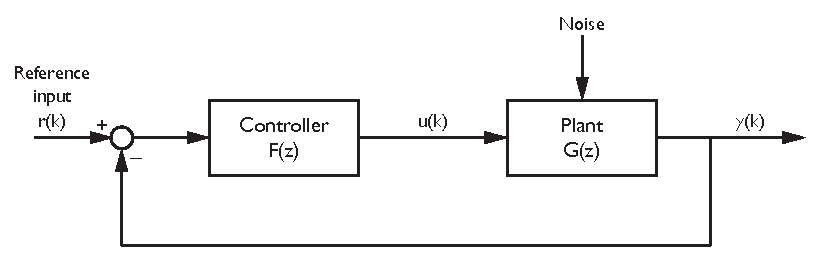
\includegraphics{../fig/closed_loop_block_diagram.pdf}
	\caption{A block diagram of an LTI system operating under feedback control.}
\end{figure}

Recently, several new approaches to identifying closed-loop systems by decoupling inputs from past noise (thus removing any bias) have been proposed. Among these approaches are the innovation estimation method proposed by Qin and Ljung \cite{qin2003closed} and the Whitening Filter Approach (WFA) proposed by Chiuso and Picci \cite{chiuso2005consistency}. The IEM pre-estimates the innovation sequence $E_f$ row-wise via a high-order Auto-Regression model with eXogeneous inputs (ARX) algorithm, which is then used to estimate $\Gamma_f$ from the extended state space model. The WFA partitions a modified version of the extended state space model row-wise and estimates $\Gamma_f$ through a multi-stage least squares followed by an SVD. It is worth noting that Chiuso and Picci concluded in \cite{chiuso2005consistency} that while all closed-loop subspace identification algorithms considered produce somewhat biased results in the presence of feedback control, these algorithms are still able to provide significant improvements over traditional SIMs when identifying closed-loop systems.

We now present an overview of the IEM procedure to identify systems operating in closed loop. We assume the following to be true:\\
\textbf{Assumption 1}: The matrix $A - KC$ is stable (i.e. its eigenvalues lie strictly within the unit circle).\\
\textbf{Assumption 2}: The pair $(A,C)$ is observable and $(A, [B \quad K])$ is controllable.\\
\textbf{Assumption 3}: The innovation sequence $e(k)$ is zero-mean white noise.\\
\textbf{Assumption 4}: The input sequence $u(k)$ is persistently exciting.

\subsection{Extended State Space Model}\label{sec:extended_state_space_model}
We again consider the combined deterministic-stochastic LTI system given in its innovation form as
\begin{subequations}
\begin{equation}x(k+1) = Ax(k) + Bu(k) + Ke(k)\end{equation}
\begin{equation}y(k) = Cx(k) + Du(k) + e(k)\end{equation}
\end{subequations}
We now assume the system input sequence $u(k)$ is determined through feedback where
\begin{equation*}
u(k) = F\big( r(k) - y(k)\big)
\end{equation*}
where $r(k)$ is the reference input. Based on the state space representation, an extended state space model can be formulated as
\begin{subequations}
\begin{equation}Y_p = \Gamma_p X_{k-p} + H_p U_p + G_p E_p\end{equation}
\begin{equation}Y_f = \Gamma_f X_k + H_f U_f + G_f E_f\end{equation}
\end{subequations}
where $p$ and $f$ denote past and future horizons, respectively. The extended observability matrix is
\begin{equation*}
\Gamma_f = \begin{bmatrix}C\\ CA\\ \vdots\\ CA^{f-1}\end{bmatrix}
\end{equation*}
and $H_f$ and $G_f$ are Toeplitz matrices of the Markov parameters of the deterministic and stochastic subsystems, respectively:
\begin{equation*}
H_f = \begin{bmatrix}
D & 0 & 0 & \cdots & 0\\
CB & D & 0 & \cdots & 0\\
CAB & CB & D & \cdots & 0\\
\vdots & \vdots  & \vdots & \ddots & \vdots\\
CA^{f-2}B & CA^{f-3}B & CA^{f-4}B & \cdots & D
\end{bmatrix}
\end{equation*}
\begin{equation*}
G_f = \begin{bmatrix}
I & 0 & 0 & \cdots & 0\\
CK & I & 0 & \cdots & 0\\
CAK & CK & I & \cdots & 0\\
\vdots & \vdots  & \vdots & \ddots & \vdots\\
CA^{f-2}K & CA^{f-3}K & CA^{f-4}K & \cdots & I
\end{bmatrix}
\end{equation*}
We arrange the input sequence into the following block Hankel form with $k$ block rows and $N$ columns:
\begin{equation*}
U_p = \begin{bmatrix}
u(0) & u(1) & \cdots & u(N-1)\\
u(1) & u(2) & \cdots & u(N)\\
\vdots & \vdots & \ddots & \vdots\\
u(k-1) & u(k) & \cdots & u(k+N-2)
\end{bmatrix}
\end{equation*}
\begin{equation*}
U_f = \begin{bmatrix}
u(k) & u(k+1) & \cdots & u(k+N-1)\\
u(k+1) & u(k+2) & \cdots & u(k+N)\\
\vdots & \vdots & \ddots & \vdots\\
u(2k-1) & u(2k) & \cdots & u(2k+N-2)
\end{bmatrix}
\end{equation*}
We construct similar matrices $Y_p$, $Y_f$, $E_p$, and $E_f$ for the output and noise sequences. The state sequences are
\begin{equation*}
X_k = \begin{bmatrix}
x(k) & x(k+1) & \cdots & x(k+N-1)
\end{bmatrix}
\end{equation*}
\begin{equation*}
X_{k-p} = \begin{bmatrix}
x(k-p) & x(k-p+1) & \cdots & x(k-p+N-1)
\end{bmatrix}
\end{equation*}


\subsection{Estimation of the Extended Observability Matrix with Innovation Estimation}
The extended state space model is
\begin{equation}\label{eq:3_extended_state_space_future_cl}
Y_f = \Gamma_f X_k + H_f U_f + G_f E_f
\end{equation}
If we partition the extended state space model row-wise, for the $i^{\mbox{th}}$ row we have
\begin{equation}\label{eq:3_extended_state_space_row}
Y_f = \begin{bmatrix}
Y_{f1}\\ Y_{f2}\\ \vdots \\ Y_{ff}
\end{bmatrix}, \qquad 
Y_{fi} = \Gamma_{fi} X_k + H_{fi} U_{fi} + G_{fi} E_{fi}
\end{equation}
where the extended observability matrix is
\begin{equation*}
\Gamma_f = \begin{bmatrix}
\Gamma_{f1}\\ \Gamma_{f2}\\ \vdots \\ \Gamma_{ff}
\end{bmatrix}, \qquad \Gamma_{fi} = CA^{i-1}
\end{equation*}
and the $i^{\mbox{th}}$ rows of $H_f$ and $G_f$ are, respectively
\begin{equation*}
H_{fi} = \begin{bmatrix} H_{i-1} & H_{i-2} & \cdots & H_1 & H_0\end{bmatrix} = \begin{bmatrix} CA^{i-2}B & CA^{i-3}B & \cdots & CB & D\end{bmatrix} 
\end{equation*}
\begin{equation*}
G_{fi} = \begin{bmatrix} G_{i-1} & G_{i-2} & \cdots & G_1 & G_0\end{bmatrix} = \begin{bmatrix} CA^{i-2}K & CA^{i-3}K & \cdots & CK & I\end{bmatrix}
\end{equation*}
Additionally, we define 
\begin{equation*}
H_{fi}^{-} = \begin{bmatrix} H_{i-1} & H_{i-2} & \cdots & H_1\end{bmatrix} = \begin{bmatrix} CA^{i-2}B & CA^{i-3}B & \cdots & CB\end{bmatrix}
\end{equation*}
\begin{equation*}
G_{fi}^{-} = \begin{bmatrix} G_{i-1} & G_{i-2} & \cdots & G_1\end{bmatrix} = \begin{bmatrix} CA^{i-2}K & CA^{i-3}K & \cdots & CK\end{bmatrix}
\end{equation*}
and derive an equivalent representation of the partitioned state space model as
\begin{equation}\label{eq:3_extended_state_space_row}
Y_{fi} = \Gamma_{fi}X_k + H_{fi}^- U_{i-1} + H_{f1}U_1 + G_{fi}^- E_{i-1} + E_{fi}
\end{equation}
By letting $A_K = A - KC$ and $B_k = B-KD$, we are able to derive an expression for the unknown state sequence $X_k$ by iterating Eq. (\ref{eq:3_extended_state_space_future_cl})
\begin{equation}\label{eq:3_state}
X_k = L_p Z_p^T + A_K^p X_{k-p}
\end{equation}
where
\begin{align*}
X_k &= \begin{bmatrix} x(k) & x(k+1) & \cdots & x(k+N-1)\end{bmatrix}\\
L_p &= \begin{bmatrix}L_p^y & L_p^u\end{bmatrix}\\
L_p^u &= \begin{bmatrix}A_K^{p-1}B_K & A_K^{p-2}B_K & \cdots & B_K\end{bmatrix}\\
L_p^y &= \begin{bmatrix}A_K^{p-1}K & A_K^{p-2}K & \cdots & K\end{bmatrix}\\
Z_p &= \begin{bmatrix} Y_p \\ U_p\end{bmatrix}
\end{align*}
Substituting Eq. (\ref{eq:3_state}) into Eq. (\ref{eq:3_extended_state_space_row}) we have
\begin{equation}\label{eq:3_extended_state_space_row_state}
Y_{fi} = \Gamma_{fi}L_p Z_p^T + \Gamma_{fi}A_{K}^p X_{k-p} + H_{fi}^- U_{i-1} + H_{f1}U_1 + G_{fi}^- E_{i-1} + E_{fi}
\end{equation}
Recalling from Assumption 1, we require the eigenvalues of $A_K$ to lie within the unit circle, so for a sufficiently large $p$, $A_K^p \approx 0$. Additionally, for convenience we assume there is no feedforward term (that is, $D = 0$) then $H_{f1} = 0$ so Eq. (\ref{eq:3_extended_state_space_row_state}) simplifies to
\begin{equation}\label{eq:3_extended_state_space_row_state_simplified}
Y_{fi} = \Gamma_{fi}L_p Z_p^T + H_{fi}^- U_{i-1} + G_{fi}^- E_{i-1} + E_{fi}
\end{equation}
or equivalently in matrix form,
\begin{equation}
Y_{fi} = \begin{bmatrix}\Gamma_{fi}L_z & H_{fi}^- & G_{fi}^-\end{bmatrix}
\begin{bmatrix}Z_p\\ U_{i-1}\\ E_{i-1}\end{bmatrix} + E_{fi}
\end{equation}
Because the future innovation sequence $E_{fi}$ is uncorrelated with the past innovation sequence $E_{i-1}$, instrumental variable matrix $Z_p$, and past output sequence $U_{i-1}$ we see that Eq. (\ref{eq:3_extended_state_space_row_state_simplified}) is formulated in such a way that we can estimate $\Gamma_{fi}$ row-wise even when the system input and past noise are correlated (i.e. the system is operating with feedback). The only requirement is that future innovation be uncorrelated with past input, which is true for both a pen and closed-loop systems. 

In order to estimate the innovation sequence $E_f$, we consider the first row of the extended state space model by setting $i = 1$ in Eq. (\ref{eq:3_extended_state_space_row_state_simplified}):
\begin{equation}
Y_{f1} = \Gamma_{f1}L_p Z_p^T + E_{1}
\end{equation}
We are able to estimate the innovation term $E_1$ through the following least squares
\begin{equation}
\hat{E}_1 = Y_{f1} - \hat{\Gamma}_{f1}\hat{L}_p Z_p
\end{equation}
with
\begin{equation}
\hat{\Gamma}_{f1}\hat{L}_p = Y_{f1} Z_p^\dagger
\end{equation}
In the more general case for $i = 1,2,\dots,f$ we have
\begin{equation}\label{eq:e_innovation_estimate}
\hat{E}_i = \begin{bmatrix}\hat{E}_{f1}\\ \hat{E}_{f2}\\ \vdots \\\hat{E}_{f1}\end{bmatrix} = 
\begin{bmatrix} \hat{E}_{i-1}\\\hat{E}_{fi}\end{bmatrix}
\end{equation}
thus using Eqs. (\ref{eq:3_extended_state_space_row_state_simplified}) and (\ref{eq:e_innovation_estimate}) we are able to estimate the innovation sequence recursively using the system input-output data. Once the innovation sequence is known, we are able to estimate the unknown coefficient matrices  through least squares as follows:
\begin{equation}\label{eq:3_iem_ls}
\begin{bmatrix}\hat{\Gamma}_{fi}\hat{L}_p & \hat{H}_{fi}^- & \hat{G}_{fi}^-\end{bmatrix} = Y_{fi}
\begin{bmatrix}Z_p\\ U_{i-1}\\ \hat{E}_{i-1}\end{bmatrix}^\dagger
\end{equation}
Computing the least squares estimate of $\hat{\Gamma}_{fi}\hat{L}_z$ row by row using Eq. (\ref{eq:3_iem_ls}), we obtain an estimate of the full matrix $\hat{\Gamma}_f\hat{L}_p$
\begin{equation*}
\hat{\Gamma}_f \hat{L}_p = \begin{bmatrix}
\hat{\Gamma}_{f1}\hat{L}_p\\ \hat{\Gamma}_{f2}\hat{L}_p\\ \vdots \\ \hat{\Gamma}_{ff}\hat{L}_p
\end{bmatrix}
\end{equation*}
from which am estimate of the column space of the extended observability matrix can be obtained via an SVD where
\begin{equation}
\hat{\Gamma}_f = US^{1/2}
\end{equation}
We follow the same procedure outlined in Section \ref{sec:3_rank_reduction} to reduce the rank of the identified system, and recover estimates of the system matrices as in Section \ref{sec:3_system_matrices}

Results from <CITE HERE> have shown a reduction in bias when identifying systems operating in closed-loop using IEM over traditional SIMs (CVA, N4SID, MOESP). Also, comparisons between the IEM and other closed-loop PEM and subspace identification techniques have shown that under the stated assumptions, estimation differences between the IEM and others are minimal and the IEM provides a consistent system estimate.
































%\subsection{Estimation of the Extended Observability Matrix by the Whitening Filter Approach}
%In order to describe the Whitening Filter Approach, we introduce the predictor form of the system:
%\begin{subequations}\label{eq:3_process}
%\begin{equation}x(k+1) = A_Kx(k) + B_Ku(k) + Ky(k)\end{equation}
%\begin{equation}y(k) = Cx(k) + Du(k) + e(k)\end{equation}
%\end{subequations}
%where $A_K = A-KC$ and $B_K = B-KD$. Because the input $u(k)$ is determined via feedback, we consider it to be correlated with past innovation $e(k)$. The state $x(k)$ of this form is the same as for the innovation form in Eq. (\ref{eq:2_innovation}), but because $A_K$ is guaranteed stable even if the original process matrix $A$ is unstable, the predictor form proves advantageous when considering open-loop unstable systems \cite{qin2006overview}.

%We are able to derive an expression for $X_k$ by iterating Eq. (\ref{eq:3_process})
%\begin{equation}\label{eq:3_state}
%X_k = L_p Z_p + A_K^p X_{k-p}
%\end{equation}
%where
%\begin{align*}
%X_k &= \begin{bmatrix} x(k) & x(k+1) & \cdots & x(k+N-1)\end{bmatrix}\\
%L_p &= \begin{bmatrix}L_p^y & L_p^u\end{bmatrix}\\
%L_p^u &= \begin{bmatrix}A_K^{p-1}B_K & A_K^{p-2}B_K & \cdots & B_K\end{bmatrix}\\
%L_p^y &= \begin{bmatrix}A_K^{p-1}K & A_K^{p-2}K & \cdots & K\end{bmatrix}\\
%Z_p &= \begin{bmatrix} Y_p^T & U_p^T\end{bmatrix}^T
%\end{align*}

%Based on the state space representation in Eq. (\ref{eq:3_process}), we construct the following modified state space model
%\begin{equation}\label{eq:3_modified_state_space_model}
%Y_f = \overline{\Gamma}_f X_k + \overline{H}_f U_f + \overline{G}_f Y_f + E_f
%\end{equation}
%with a modified extended observability matrix given by
%\begin{equation}\label{eq:3_updated_extended_observability}
%\overline{\Gamma}_f = \begin{bmatrix}C\\ CA_K\\ \vdots\\ CA_K^{f-1}\end{bmatrix}
%\end{equation}
%and Toeplitz matrices $\overline{H}_f$ and $\overline{G}_f$ given by
%\begin{subequations}\label{eq:3_updated_toeplitz}
%\begin{equation}
%\overline{H}_f = \begin{bmatrix}
%D & 0 & 0 & \cdots & 0\\
%CB_K & D & 0 & \cdots & 0\\
%CA_KB_K & CB_K & D & \cdots & 0\\
%\vdots & \vdots  & \vdots & \ddots & \vdots\\
%CA_K^{f-2}B_K & CA_K^{f-3}B_K & CA_K^{f-4}B_K & \cdots & D
%\end{bmatrix}
%\end{equation}
%\begin{equation}
%\overline{G}_f = \begin{bmatrix}
%0 & 0 & 0 & \cdots & 0\\
%CK & 0 & 0 & \cdots & 0\\
%CA_KK & CK & 0 & \cdots & 0\\
%\vdots & \vdots  & \vdots & \ddots & \vdots\\
%CA_K^{f-2}K & CA_K^{f-3}K & CA_K^{f-4}K & \cdots & 0
%\end{bmatrix}
%\end{equation}
%\end{subequations}

%Substituting Eq. (\ref{eq:3_state}) into Eq. (\ref{eq:3_modified_state_space_model}), we have
%\begin{equation}\label{eq:3_modified_state_space_model_with_state}
%Y_f = \overline{\Gamma}_f L_p Z_p + \overline{\Gamma}_f A_K^p X_{k-p} + \overline{H}_f U_f + \overline{G}_f Y_f + E_f
%\end{equation}
%If we assume that the eigenvalues of $A_K$ lie strictly within the unit circle, for a sufficiently large $p$, $A_K^p \approx 0$ so Eq. (\ref{eq:3_modified_state_space_model_with_state}) becomes
%\begin{equation}\label{eq:3_modified_state_space_model_with_state_no_AK}
%Y_f = \overline{\Gamma}_f L_p Z_p + \overline{H}_f U_f + \overline{G}_f Y_f + E_f
%\end{equation}
%Partitioning Eq. (\ref{eq:3_modified_state_space_model_with_state_no_AK}) row-wise, we have
%\begin{equation}\label{eq:3_partitioned_modified_state_space_model}
%Y_{fi} = \overline{\Gamma}_{fi} L_p Z_p + \overline{H}_{fi} U_{fi} + \overline{G}_{fi} Y_{fi} + E_{fi}
%\end{equation}
%where
%\begin{align*}
%\overline{\Gamma}_{fi} &= CA_K^{i-1}\\
%\overline{H}_{fi} &= \begin{bmatrix} CA_K^{i-2}B_K & CA_K^{i-3}B_K & \cdots & CB_K & D\end{bmatrix}\\
%\overline{G}_{fi} &= \begin{bmatrix} CA_K^{i-2}K & CA_K^{i-3}K & \cdots & CK & 0\end{bmatrix}
%\end{align*}

%Using least squares, we estimate $\overline{\Gamma}_{fi}L_p$ for $i = 1, 2, \dots, f$, which then forms $\widehat{\overline{\Gamma}_f L_p}$































